% CPC manuscript. The TeX source is the paper. The org file is not.
\documentclass[preprint,12pt]{elsarticle}
\usepackage{graphicx}
\journal{Computer Physics Communications}
\usepackage{iftex}
\ifPDFTeX\usepackage[utf8]{inputenc}\usepackage[T1]{fontenc}\usepackage{lmodern}\else\usepackage{fontspec}\fi
\usepackage{microtype}
\makeatletter
% The class footer box is followed by a space token.
% The output routine then packs that box to \textwidth, and the space makes the line 2.6pt overfull.
\def\ps@pprintTitle{%
\let\@oddhead\@empty
\let\@evenhead\@empty
\def\@oddfoot{%
\hbox to \textwidth{%
\ifnopreprintline\relax\else
\@myfooterfont
\ifx\@elsarticlemyfooteralign\@elsarticlemyfooteraligncenter
\hfil\@elsarticlemyfooter\hfil
\else
\ifx\@elsarticlemyfooteralign\@elsarticlemyfooteralignleft
\@elsarticlemyfooter\hfill{}%
\else
\ifx\@elsarticlemyfooteralign\@elsarticlemyfooteralignright
{}\hfill\@elsarticlemyfooter
\else
Preprint submitted to \ifx\@journal\@empty
Elsevier%
\else\@journal\fi\hfill\@date\fi
\fi
\fi
\fi
}%
}%
\let\@evenfoot\@oddfoot}
\makeatother
\usepackage{amssymb,amsmath}
\usepackage{booktabs}
\usepackage{listings}
\usepackage{xurl}
\usepackage{seqsplit}
\usepackage{algorithm}
\usepackage{algpseudocode}
\usepackage{xcolor}
\usepackage{hyperref}
\usepackage{xr-hyper}
\externaldocument{rg_supp}
\input{affilfix}
% Release pin. Package version and the commit that produced Section 6.
% TODO(DOI): mint the Zenodo version DOI for readcon-core 0.17.2; concept DOI kept below.
\newcommand{\readconversion}{0.17.2}
\newcommand{\readconcommit}{5c849d1b1d3dede45e20665c5730abe3d5f18f84}
\newcommand{\readconcommitshort}{5c849d1}
\newcommand{\readcondoi}{TODO(DOI)}
\lstset{
basicstyle=\ttfamily\footnotesize,
breaklines=true,
columns=fullflexible,
keepspaces=true,
showstringspaces=false,
frame=none,
aboveskip=0.6em,
belowskip=0.4em
}
\hypersetup{colorlinks=true,linkcolor=black,citecolor=black,urlcolor=blue!50!black}
\date{\today}
\title{CON 3.1: a versioned restart state for saddle searches}
\hypersetup{
 pdfauthor={Rohit Goswami},
 pdftitle={CON 3.1: a versioned restart state for saddle searches},
 pdfkeywords={restart, specification, saddle search, conformance, nudged elastic band},
 pdfsubject={},
 pdflang={English}}
\begin{document}

\begin{frontmatter}

\input{authors.tex}

\begin{abstract}
A saddle search resumes from a geometry file that must keep a per-axis mask, a persistent atom identifier, a declared velocity unit, binary64 coordinates and a versioned grammar.
An ASE POSCAR round trip drops the adatom height constraint, and the resumed climbing-image band finishes \(70.2\,\mathrm{meV}\) below the uninterrupted barrier of \(0.644561366\,\mathrm{eV}\).
CON 3.1 is that grammar for the text eOn already writes, checked by a conformance corpus and implemented once behind C, C++, Python, Julia and Fortran.
Twenty-five writer-reader pairs resume that band from each other's restart files.
On \(10{,}000\) frames, a full-field Python read finishes at \(0.154\) times MDAnalysis H5MD, \(1.73\) times chemfiles XYZ and \(51.9\) times h5py; coordinate accumulation alone changes those ratios to \(0.160\), \(1.63\) and \(36.4\).
A warm native read on readcon-core~\readconversion{} (commit~\readconcommitshort{}) takes \(9.70\,\mu\mathrm{s}\) per frame.
\end{abstract}

\begin{keyword}
restart \sep specification \sep saddle search \sep conformance \sep nudged elastic band
\end{keyword}

\begin{highlights}
\item A restart file needs a mask, an id, a time unit, binary64 coordinates and a version.
\item One masked slab loses part of that state in every common format tested.
\item An ASE POSCAR resume drops a height constraint and ends 70.2 meV lower.
\item Five extended XYZ readers return four answers for one file.
\item Twenty-five writer-reader pairs resume the barrier from each other's restart files.
\end{highlights}

\end{frontmatter}

\noindent\begin{minipage}{5cm}
\centering
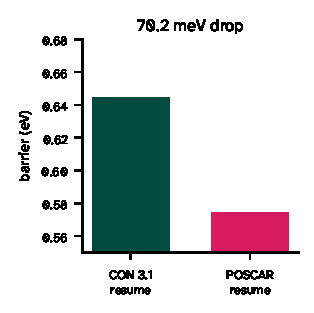
\includegraphics[width=5cm]{figures/generated/toc.pdf}\\[0.4em]
{\footnotesize TOC. CON~3.1 keeps the mask the POSCAR route drops; the resumed band stays at \(0.644561366\,\mathrm{eV}\), \(70.2\,\mathrm{meV}\) above that POSCAR resume.}
\end{minipage}

{\bf PROGRAM SUMMARY}

\begin{small}
\noindent
\textit{Program title:} readcon-core\\
\textit{CPC Library link to program files:} (to be added by Technical Editor)\\
\textit{Developer's repository link:} \url{https://github.com/lode-org/readcon-core}\\
\textit{Licensing provisions:} MIT\\
\textit{Code Ocean capsule:} none\\
\textit{References:} see the bibliography of this paper\\
\textit{Programming language:} Rust, C, C++, Python, Julia, Fortran 2008\\
\textit{Supplementary material:} specification, grammar, conformance corpus, and the tables behind the measurements\\

\textit{Nature of problem:}
Rare-event campaigns stop and resume from a stored geometry.
The formats in common use each drop part of the resume state: a per-axis mask, a persistent atom identifier, the velocity time unit, binary64 coordinates, or the periodic flags.
Readers of one format also disagree with each other, so the resumed search runs on a different surface.

\textit{Solution method:}
CON 3.1 is a versioned grammar.
A reader of a known major accepts a later minor, keeps unknown keys, and rejects an unknown major.
Every velocity block declares its time unit.
The default writer emits the shortest decimal that parses back to the same binary64 value.
A corpus of legal and illegal frames decides what a conforming reader accepts.
One Rust core sits behind one C interface, and eOn 3.6.0 reads and writes CON through it.
The companion store keeps that text, indexes composition, energy and forces, recognises gzip and zstd wrappers of the same text, and ingests frames from several MPI ranks.
Its map starts at 2 GiB, and the caller can raise that limit.

\textit{Additional comments including restrictions and unusual features:}
A CON 3.1 frame stores Cartesian coordinates, the cell lengths and angles, the periodic flags, a per-axis mobility mask and a persistent atom identifier.
From minor 1, a velocity block names its time unit.
The same row layout carries forces, per-atom energies, charges, spins, magnetic moments, displacements and spreads.
The JSON header carries the grammar version, and it carries an energy, a potential name and band indices when the writer recorded them.
gzip and zstd wrappers of that text are part of the grammar.
The frame does not store the displacement history of a quasi-Newton update or of a FIRE step, so an optimiser that needs those vectors takes a different step after a resume.
A band is a sequence of frames.
It is not one frame that holds the optimiser state.
Files written by earlier eOn releases are grammar version 1: column 4 is 0 or 1 and the JSON line is absent.
A 3.1 reader accepts them under that column rule, and a 3.1 writer emits the versioned header.
The memory-mapped store keeps each CON text and indexes on composition, energy and maximum force.
The map starts at 2 GiB and the caller can raise it.
Thread and peer timings used \readconversion{} (commit~\readconcommitshort{}).
The MPI timings used readcon-core 0.17.0 (commit af8aabb).
The store timings used readcon-core 0.16.2 and readcon-db 0.1.8.
\end{small}



\section{Introduction}
\label{sec:introduction}
Rare-event methods turn a potential energy surface into rates. Transition state theory
\cite{eyringActivatedComplexChemical1935,vineyardFrequencyFactorsIsotope1957,hanggiReactionrateTheoryFifty1990}
reduces kinetics to saddle points. These are located by the nudged elastic band
\cite{jonssonNudgedElasticBand1998,henkelmanClimbingImageNudged2000,henkelmanImprovedTangentEstimate2000,asgeirssonNudgedElasticBand2021},
by minimum-mode followers \cite{henkelmanDimerMethodFinding1999,kastnerSuperlinearlyConvergingDimer2008,olsenComparisonMethodsFinding2004},
and by string methods \cite{eStringMethodStudy2002,petersGrowingStringMethod2004}.
The results are chained into adaptive kinetic Monte Carlo and accelerated dynamics
\cite{henkelmanLongTimeScale2001,xuAdaptiveKineticMonte2008,voterExtendingTimeScale2002,perezLongtimeDynamicsThrough2016}.
None of these is a single calculation. A long-timescale run in eOn \cite{chillEonSoftwareLong2014,rohitgoswamiTheochemuieonV3602026}
spawns thousands of saddle searches, often on volunteer or distributed resources
\cite{andersonBoincSystemPublicresource2005,pedersenDistributedImplementationAdaptive2010}. It restarts them, and it passes
geometries between Python drivers \cite{larsenAtomicSimulationEnvironmenta2017,hermesSellaOpensourceAutomationfriendly2022},
C++ engines and Fortran electronic structure codes \cite{kresseEfficiencyAbinitioTotal1996}.
The geometry file is therefore not an export format. It is the \emph{restart state} of the
algorithm.

That restart state has requirements that general-purpose formats were not designed for. A
surface saddle search fixes the slab and lets an adatom move only along the surface normal. It
therefore needs mobility per atom \emph{and per axis}. Mode following and AKMC bookkeeping need
atom identity that survives reordering. Dynamics-based steps need velocities whose unit is
declared. eOn's natural time unit, \((\mathrm{amu}\,\mathrm{\AA}^2/\mathrm{eV})^{1/2}\), is \(10.180505710759414\,\mathrm{fs}\) for the CODATA 2018 constants \cite{tiesingaCodataRecommendedValues2021}.
The square of that value, \(103.64269652680504\), is the factor in the kinetic energy when the same numbers are read as \(\text{\AA}/\mathrm{fs}\). A converged
band restarted from rounded coordinates is no longer converged, so coordinates must round-trip
in binary64 \cite{ieeecomputersocietyIeeeStandardFloatingpoint2019,clingerHowReadFloating1990,steeleHowPrintFloatingpoint1990,adamsRyFastFloattostring2018}.
Finally, two readers given the same bytes must agree, which needs a versioned grammar rather than a
convention.

Existing formats meet some of these requirements, but none meets all of them. Extended XYZ carries
per-axis masks only through an ASE-specific column. It writes coordinates at eight decimals by
default, which moves positions by up to \(10^{-9}\)\,\AA{} on a round trip, and it has no version
or velocity unit. H5MD \cite{buylH5mdStructuredEfficient2014,folkOverviewHdf5Technology2011}
records identity, velocities and box, but it has no per-axis constraint field and treats units
as optional attributes. TNG \cite{spangbergTrajectoryNgPortable2011,lundborgEfficientExtensibleFormat2014}
and NetCDF trajectories \cite{rewNetcdfInterfaceScientific1990} target compressed MD output, not
optimiser restarts. ASE's own trajectory file is lossless within ASE, but it is defined by its
Python implementation and cannot be read from the C++ and Fortran codes that do the work. Readers
of the original CON format drift too. We found that the ASE copy of the eOn writer currently
fails outright on per-axis constraints, and that a POSCAR round trip silently drops them. Toolkits
such as chemfiles and MDAnalysis
\cite{frauxChemfileschemfilesVersion01042023,gowersMdanalysisPythonPackage2016}
widen \emph{access}, but they inherit whatever each format leaves undefined.

\subsection{Contribution}
We do not propose another container. We make the format eOn already uses into a
\emph{specification with a test suite} and give it a single implementation:
\begin{enumerate}
\item \textbf{CON 3.1}, a versioned grammar that specifies per-axis mask bits, a persistent atom
  identifier, velocities in a declared unit, and shortest round-trip binary64 output
  \cite{andryscoPrintingFloatingpointNumbers2016,loitschPrintingFloatingpointNumbers2010}.
\item \textbf{An executable conformance corpus}. Any reader, ours or not, can be checked
  against it. Agreement between readers is then something we test, not something we assume.
\item \textbf{One core, many bindings}. A Rust library behind a C ABI serves C++, Python, Julia
  \cite{bezansonJuliaFreshApproach2017} and Fortran. Per-language behaviour cannot drift, because
  there is only one parser. This follows the precedent set by chemfiles
  \cite{frauxChemfileschemfilesVersion01042023}. eOn 3.6.0 reads and writes through it.
\end{enumerate}
We show each failure above as a reproducible case and show that CON 3.1 removes it. We then
demonstrate bit-exact restart of a masked, asymmetric NEB across languages. Throughput comes last.
We report it against the peer readers, with the cases where readcon is slower stated plainly
\cite{hoeflerScientificBenchmarkingParallel2015,kaliberaRigorousBenchmarkingReasonable2013}.
Section \ref{sec:requirements} measures the five requirements on one frame, Section \ref{sec:format} states the grammar, and Section \ref{sec:conformance} is the corpus and the extended XYZ disagreement.
Section \ref{sec:implementation} is the reader and the store.
Section \ref{sec:cases} resumes one band through every route we completed, and Section \ref{sec:performance} reports threads, peers, MPI and the store.
Those timings name the build that was clocked.

\section{Requirements and the failure each one closes}
\label{sec:requirements}
Table \ref{tab:requirements} states five requirements.
Each is a field a later step reads.
The frame stores the geometry and its labels.
It does not store the short history of a quasi-Newton update \cite{nocedalUpdatingQuasinewtonMatrices1980,sheppardOptimizationMethodsFinding2008} or of a FIRE step \cite{bitzekStructuralRelaxationMade2006}.
Section \ref{sec:cases} measures that difference on one band.

\begin{table}[ht]
\centering
\small
\caption{Requirements on a restart state, the step that reads each field, and the failure measured when the field is missing.}
\label{tab:requirements}
\begin{tabular}{p{0.22\linewidth}p{0.32\linewidth}p{0.36\linewidth}}
\toprule
Requirement & Step that reads it & Failure measured here \\
\midrule
R1, per-axis mask & Surface search, prefactor & Height constraint dropped; barrier \(-70.2\,\mathrm{meV}\) \\
R2, persistent id & Band and event table & Id lost on completed foreign round trips \\
R3, declared time unit & Dynamics & Kinetic energy scaled by \(103.642696\) \\
R4, binary64 geometry, cell, periodicity & Resume of a search & \(10^{-9}\) to \(10^{-6}\,\text{\AA}\), or periodicity rewritten \\
R5, versioned grammar & Any second reader & One file, four answers from five readers \\
\bottomrule
\end{tabular}
\end{table}

R1 is a mask for each Cartesian axis of each atom.
R2 is an integer stored on the row, so a later frame finds the same atom after the file groups rows by element.
R3 is a time unit written in the file.
R4 is coordinates, cell and periodic flags that read back as the values written.
R5 is a grammar with a major and a minor, a rule for what a later minor adds, and a corpus that decides disputes.

\subsection{One frame through each format}
The frame is a Pt(100) slab with one adatom: the bottom atoms held on every axis, the adatom held in \(z\), identifiers that are not the row order, and velocities in the natural unit.
Section \ref{sec:supp-failure} gives the coordinates, the identifiers and the grading rules.
Each row of Table \ref{tab:survey} writes that frame with one library and reads it with another.
The libraries are ASE 3.29.0 \cite{larsenAtomicSimulationEnvironmenta2017}, chemfiles 0.10.4 \cite{frauxChemfileschemfilesVersion01042023}, MDAnalysis 2.10.0 \cite{gowersMdanalysisPythonPackage2016,gowersMdanalysismdanalysisRelease21002025}, and h5py 3.16.0 where the route needs it.
POSCAR selective dynamics is the per-axis mask in the VASP ionic restart \cite{kresseEfficientIterativeSchemes1996,kresseEfficiencyAbinitioTotal1996}.

\input{figures/generated/survey_table}

The CON 3.1 row keeps every field.
Extended XYZ written and read by ASE returns the mask, the identifiers and the time unit because both sides share ASE's column names and ASE's internal unit.
The extended XYZ grammar does not define those names, so chemfiles drops the mask and MDAnalysis drops the mask and the identifiers.
The ASE writer prints a fixed number of decimals and the coordinates move by up to \(4.7\times10^{-9}\,\text{\AA}\).
chemfiles writing the same frame moves them by \(4.9\times10^{-6}\,\text{\AA}\) and returns every axis periodic.
MDAnalysis returns single-precision coordinates, a shift of \(2.2\times10^{-7}\,\text{\AA}\).
The ASE trajectory keeps the mask and the coordinates exactly and drops the identifier.
Its time unit is the library's unit, which the file does not name.
The ASE POSCAR writer turns the held slab into a different mask and writes the adatom free.
POSCAR has no atom identifier and no open axis.
H5MD written by MDAnalysis declares the velocity unit, writes no mask and no identifier, stores single-precision coordinates, and marks the open \(z\) axis periodic \cite{buylH5mdStructuredEfficient2014}.
An extra array carries a mask only when every reader agrees on its name and type.
Section \ref{sec:cases} attaches that array and shows which readers return it.
The ASE eon reader rejects a CON frame that contains a velocity block.
Given coordinates alone it freezes every masked atom on every axis, drops the identifiers, and returns no periodic axis.
The ASE eon writer cannot express a per-axis constraint, so that route produces no file.
Table \ref{tab:compare} places the same checkpoint next to trajectory containers and structure archives.

\section{The CON 3.1 specification}
\label{sec:format}
A CON file is a sequence of text frames.
Listing \ref{lst:frame} is the survey frame of Table \ref{tab:survey}.
Section \ref{sec:supp-failure} states how that frame was built.

\begin{lstlisting}[caption={The survey frame. Line 1 is an empty user line. Line 2 declares the version, the units and the periodicity. Identifiers are 17, 3, 11, 5, 23, 2, 13, 7 and 41.},label={lst:frame}]

{"con_spec_minor":1,"con_spec_version":3,"pbc":[true,true,false],"sections":["velocities"],"units":{"energy":"eV","length":"angstrom","mass":"amu","time":"(amu*angstrom^2/eV)^0.5"}}
5.5437171645025325e0 5.5437171645025325e0 1.396e1
9e1 9e1 9e1


1
9
1.95084e2
Pt
Coordinates of Component 1
1.386493891622963e0 1.3858827980505872e0 5.999231933623632e0 7 17
4.158528117245317e0 1.3861213257350742e0 5.999813419553613e0 7 3
1.3860627284818523e0 4.158248487145931e0 6.000055839372117e0 7 11
4.1574916113945894e0 4.157781657328241e0 6.000983049344183e0 7 5
-2.684564058587828e-4 6.114378220263555e-4 7.959946638798572e0 0 23
2.7723693731828494e0 2.842894752666141e-4 7.959407544708384e0 0 2
7.71950084012911e-4 2.772315330818269e0 7.960901835964954e0 0 13
2.772542023981585e0 2.7723297461317795e0 7.959545089014511e0 0 7
1.3867197337624881e0 1.3861370701026228e0 9.760314828133515e0 4 41

Pt
Velocities of Component 1
0e0 0e0 0e0 7 17
0e0 0e0 0e0 7 3
0e0 0e0 0e0 7 11
0e0 0e0 0e0 7 5
-4.419216359135741e-3 -3.1227306022671786e-3 5.3252274765567134e-3 0 23
-1.9411746848912532e-3 -4.423003635856234e-3 4.825314186834311e-3 0 2
-5.72219106757806e-3 -3.294382313545619e-3 -3.7362717028046195e-4 0 13
-1.8722607532418165e-3 8.120539032663098e-4 2.918400292950336e-3 0 7
-1.6020339068388144e-3 4.319885827377455e-3 0e0 4 41
\end{lstlisting}

Line 1 is free text.
Line 2 is one JSON object \cite{brayJavascriptObjectNotation2017}.
Lines 3 and 4 are the cell lengths and the angles in degrees.
The type count, the per-type counts and the masses follow.
Each coordinate row is \(x\), \(y\), \(z\), the mask and the identifier.
Lengths and angles rebuild the box with \(a\) along \(x\) and \(b\) in the \(xy\) plane,
\begin{equation}
\mathbf{a}=a\,\hat{\mathbf{x}},\qquad
\mathbf{b}=b\cos\gamma\,\hat{\mathbf{x}}+b\sin\gamma\,\hat{\mathbf{y}},
\end{equation}
after which \(\mathbf{c}\) is fixed by \(\alpha\) and \(\beta\) so the cell is right-handed \cite{bekkerUnificationBoxShapes1997}.
When line 2 carries lattice vectors, those rows are the cell.
A missing periodicity flag means periodic on every axis.

\paragraph{R1, the mask.}
Column 4 is the integer of Table \ref{tab:mask}.
Mask 0 is free, mask 4 fixes \(z\) only, and mask 7 fixes every axis.
A float spelling, a sign, or a value outside 0 to 7 is an illegal flag.
Under version 1 the column is 0 or 1, so masks 4 and 7 cannot be stored as written.

\begin{table}[ht]
\centering
\small
\caption{Mask bits from version 2. Version 1 stores 0 (free) or 1 (fixed on \(x\), \(y\) and \(z\)) in the same column.}
\label{tab:mask}
\begin{tabular}{ccc}
\toprule
Bit & Axis & Value \\
\midrule
0 & \(x\) & 1 \\
1 & \(y\) & 2 \\
2 & \(z\) & 4 \\
\bottomrule
\end{tabular}
\end{table}

\paragraph{R2, the identity.}
Column 5 is an integer from 0 through \(2^{64}-1\).
Writers emit identifiers unique within a frame.
A missing identifier column takes the zero-based row index.

\paragraph{R3, the time unit.}
From minor 1, a velocity block declares \texttt{units.time}.
The natural unit is spelled \texttt{(amu*angstrom\textasciicircum{}2/eV)\textasciicircum{}0.5}.
The reference reader converts that spelling to \(10.180505710759414\,\mathrm{fs}\) for the CODATA 2018 constants \cite{tiesingaCodataRecommendedValues2021}.
The square of the printed value is \(103.64269652680504\).
Versions 1, 2 and 3.0 are read in the natural unit.
An fs label on those older files is not trusted: producers of that era wrote natural-unit numbers under an fs label \cite{rohitgoswamiTheochemuieonV3602026}.

\paragraph{R4, the numbers.}
Readers convert each finite decimal to binary64 with correct rounding \cite{ieeecomputersocietyIeeeStandardFloatingpoint2019,clingerHowReadFloating1990}.
The default writer prints the shortest decimal that parses back to the same value \cite{adamsRyFastFloattostring2018,loitschPrintingFloatingpointNumbers2010}.
Six fixed decimals are an optional writer mode.
gzip and zstd wrap the same bytes, and a reader recognises the wrapper by content \cite{deutschGzipFileFormat1996,colletZstandardCompressionApplicationzstd2021}.
A conforming reader accepts the compressed file and returns the same frames.

\paragraph{R5, the version.}
Table \ref{tab:keys} lists the reserved keys of the JSON line.
A reader accepts a later minor of a known major, keeps an unknown key on rewrite, skips an unknown section whose width is declared, and rejects an unknown major.
H5MD uses the same split for its version pair \cite{buylH5mdStructuredEfficient2014}.
Table \ref{tab:versions} is the history of the grammar.
Table \ref{tab:sections} is the sections reserved at minor 1.

The mask integer \(m\in\{0,\ldots,7\}\) for version \(\ge 2\) is the bit union
\begin{equation}
\label{eq:mask}
m = b_x + 2 b_y + 4 b_z,\qquad b_\alpha\in\{0,1\},
\end{equation}
so axis \(\alpha\) is fixed when \(b_\alpha=1\).
Under version 1 the same column stores only \(0\) (free) or \(1\) (fixed on every axis).
A reader that meets a velocity block at minor \(\ge 1\) requires a declared time unit \(u\); otherwise it rejects the file.
Acceptance of a later minor of a known major, with unknown keys retained, is
\begin{equation}
\label{eq:version}
\mathrm{accept}(M.m) \iff M\in\mathcal{M}_{\mathrm{known}}\ \mathrm{and}\ m\ge 0,
\end{equation}
where \(\mathcal{M}_{\mathrm{known}}=\{1,2,3\}\) in this release.
Algorithm~\ref{alg:accept} is that decision procedure.

\begin{algorithm}[ht]
\caption{Accept or reject one CON frame}
\label{alg:accept}
\begin{algorithmic}[1]
\Require bytes of one frame, known majors \(\mathcal{M}_{\mathrm{known}}\)
\Ensure accepted fields, or reject
\State Unwrap gzip or zstd if present; parse the header for major \(M\) and minor \(m\)
\If{\(M\notin\mathcal{M}_{\mathrm{known}}\)}
  \State \textbf{reject} unknown major
\EndIf
\State Read type counts, cell, periodic flags, and each atom row \((x,y,z,m_{\mathrm{col}},\mathrm{id})\)
\If{\(M\ge 2\) and \(m_{\mathrm{col}}\notin\{0,\ldots,7\}\)}
  \State \textbf{reject} illegal mask
\ElsIf{\(M=1\) and \(m_{\mathrm{col}}\notin\{0,1\}\)}
  \State \textbf{reject} illegal mask
\EndIf
\State Decode fixed axes from \(m_{\mathrm{col}}\) by Eq.~\eqref{eq:mask} (or the version-1 rule)
\If{a velocity section is present and \(m\ge 1\) and \texttt{units.time} is absent}
  \State \textbf{reject} missing time unit
\EndIf
\State Keep unknown JSON keys; skip unknown sections whose width is declared
\State \textbf{accept} the frame
\end{algorithmic}
\end{algorithm}
The reader rules are Table \ref{tab:rules}.
The grammar of one frame is the listing in Section \ref{sec:appendix-abnf}.
The prose specification wins where the listing and the prose disagree.

\begin{table}[ht]
\centering
\footnotesize
\caption{Reserved metadata keys of the JSON header line.}
\label{tab:keys}
\begin{tabular}{ll@{\hspace{1.4em}}ll}
\toprule
Key & Type & Key & Type \\
\midrule
\texttt{con\_spec\_version} & int & \texttt{neb\_bead} & int \\
\texttt{con\_spec\_minor} & int & \texttt{neb\_band} & int \\
\texttt{section\_arity} & object & \texttt{convergence\_fmax} & number \\
\texttt{sections} & array & \texttt{convergence\_energy} & number \\
\texttt{validate} & bool & \texttt{converged} & bool \\
\texttt{generator} & string & \texttt{fmax} & number \\
\texttt{units} & object & \texttt{bonds} & array \\
\texttt{pbc} & array & \texttt{storage\_dtypes} & object \\
\texttt{lattice\_vectors} & array & \texttt{chemfiles\_atom\_names} & array \\
\texttt{energy} & number & \texttt{chemfiles\_atom\_types} & array \\
\texttt{potential} & object & \texttt{chemfiles\_atom\_properties} & array or object \\
\texttt{frame\_index} & int & \texttt{time} & number \\
\texttt{timestep} & number & & \\
\bottomrule
\end{tabular}
\end{table}

\begin{table}[ht]
\centering
\small
\caption{CON versions. The date is the day the rule was fixed.}
\label{tab:versions}
\begin{tabular}{@{}llp{0.55\linewidth}@{}}
\toprule
Version & Date & Change \\
\midrule
1 & eOn text & Column 5 present. Column 4 is 0 or 1. No JSON line. \\
2 & 2026-03-25 & A JSON header line, identifiers, bit masks, declared sections. \\
3.0 & 2026-06-27 & Length and energy units required. No minor. \\
3.1 & 2026-10-11 & Minor 1. A velocity block declares the time unit. \\
\bottomrule
\end{tabular}
\end{table}

\begin{table}[ht]
\centering
\small
\caption{Reserved sections at minor 1. Each data row carries its values, then the mask and the identifier.}
\label{tab:sections}
\begin{tabular}{lll}
\toprule
Section & Values & Rule \\
\midrule
Velocities & \(v_x\, v_y\, v_z\) & Time unit from minor 1 \\
Forces & \(f_x\, f_y\, f_z\) & \\
Energies & one value & Name \texttt{energies} \\
Charges & one value & \\
Spins & one value & \\
Magmoms & \(m_x\, m_y\, m_z\) & \\
Displacements & \(d_x\, d_y\, d_z\) & \texttt{units.length} \\
Spreads & \(s_x\, s_y\, s_z\) & \texttt{units.length}, each at least 0 \\
\bottomrule
\end{tabular}
\end{table}

\subsection{What the text costs}
\label{sec:rationale}
eOn has written this text since its first releases \cite{chillEonSoftwareLong2014}.
Those campaigns store grammar version 1: column 4 is 0 or 1 and there is no JSON line (Table \ref{tab:versions}).
A 3.1 reader accepts that file under the version-1 column rule.
A 3.1 writer emits the versioned header, which is a different file.
The bytes do not depend on endianness \cite{pedersenDistributedImplementationAdaptive2010}.
A diff of a text checkpoint shows a changed mask or identifier.
The JSON line takes a new key without a new grammar, and a reader keeps a key it does not know \cite{brayJavascriptObjectNotation2017}.

Table \ref{tab:sizes} is the byte cost of one 218-atom frame and of that frame repeated \(10{,}000\) times, raw and after gzip at level 6.
The repeated file is the same text, so its gzip column is smaller than the gzip column of a trajectory whose frames differ.
One CON frame is \(41.99\) bytes per atom, against \(83.64\) for extended XYZ written by ASE with the mask column, \(314.39\) for one H5MD frame written by MDAnalysis, and \(95.40\) for one H5MD frame written by h5py with binary64 positions, a mask dataset and an identifier dataset.
At \(10{,}000\) copies the raw CON cost stays \(41.99\) bytes per atom.
H5MD amortises its container and falls to \(12.61\) and \(24.04\) bytes per atom.
gzip of the repeated CON file reaches \(0.39\) bytes per atom.
H5MD is the record for a long trajectory \cite{buylH5mdStructuredEfficient2014}.
CON is the record for the checkpoint, where one frame has to keep the mask, the identifier and the unit.

\input{figures/generated/sizes_table}

\section{Conformance and drift}
\label{sec:conformance}
The corpus is the executable form of the grammar.
It holds 10 legal files and 8 illegal files, split as in Table \ref{tab:corpus}.
A conforming reader accepts the first group and rejects the second.
The conformance goldens are Python, C, Fortran and Julia.
There is no C++ golden.
C++ joins the twenty-five writer-reader pairs in Section \ref{sec:cases}.
That test is separate from the corpus.

\begin{table}[ht]
\centering
\small
\caption{Conformance corpus. Counts are the committed manifest summary.}
\label{tab:corpus}
\begin{tabular}{@{}lrp{0.55\linewidth}@{}}
\toprule
Category & Files & What a reader must do \\
\midrule
Header and units & 2 & Accept a version-2 header and a version-3 units line. \\
Column-4 masks & 5 & Accept version-1 full freeze and version-2 per-axis flags. \\
Empty frame & 3 & Accept a type count of zero. \\
Illegal & 8 & Reject the file. \\
\bottomrule
\end{tabular}
\end{table}

Table \ref{tab:versionsafety} applies R3 and R5 to seven headers of one velocity frame.
Python and C follow the rule on each row.
They reject a minor-1 velocity block with no time unit, an unknown major, a missing version and a mask of 9, and they keep an unknown key from a later minor.
The ASE eon reader has no version rule.
Given the coordinate block, it accepts all seven, including the illegal mask and the unknown major.

\input{figures/generated/versionsafety_table}

Extended XYZ has a published layout and parsers in several languages, so it is the text format to compare on R5.
Table \ref{tab:drift} gives five readers seven three-atom files.
The readers are ASE 3.29.0, libAtoms through its C path and its Python path, chemfiles 0.10.4, and MDAnalysis 2.10.0.
On the reference frame the five readers return four outcomes: ASE and the libAtoms C path accept it, the libAtoms Python path changes the mask booleans, chemfiles moves one coordinate by one unit in the last place and returns no mask, and MDAnalysis returns single precision with no mask and no identifiers.
The correctly rounded binary64 value of the coordinate \(2.7718585822512662\) has bit pattern \texttt{40062cc4313f3fb9}; chemfiles returns \texttt{40062cc4313f3fb8} (Section \ref{sec:supp-failure}).
A Fortran exponent \texttt{6.0d0} is read by the libAtoms C path, returned as NaN by the libAtoms Python path, and rejected by the other three.
A plain comment line is non-periodic to ASE, periodic to the libAtoms C path, and rejected by the libAtoms Python path.
The readers follow their own documentation.
The grammar does not decide these cases, and the formats share no corpus that would.

\input{figures/generated/drift_table}

\section{Reference implementation}
\label{sec:implementation}
The reference reader and writer is the Rust core behind the C interface.
The concept record covers the line of releases \cite{goswamiReadconcoreConConvel2026}.
Figure \ref{fig:architecture} is the layering.
One Rust core parses and writes.
One C interface is the waist every other caller uses.
C++ wraps it for eOn 3.6.0.
Python exposes array views \cite{harrisArrayProgrammingNumpy2020}.
Julia calls the C interface \cite{bezansonJuliaFreshApproach2017}.
Those writer-reader pairs call that interface from Fortran 2008.
chemfiles took the same route for trajectories: one core and several language bindings \cite{frauxChemfileschemfilesVersion01042023}.
Decimal fields go through one correctly rounded conversion on that shared path \cite{adamsRyFastFloattostring2018}.

\begin{figure}[ht]
\centering
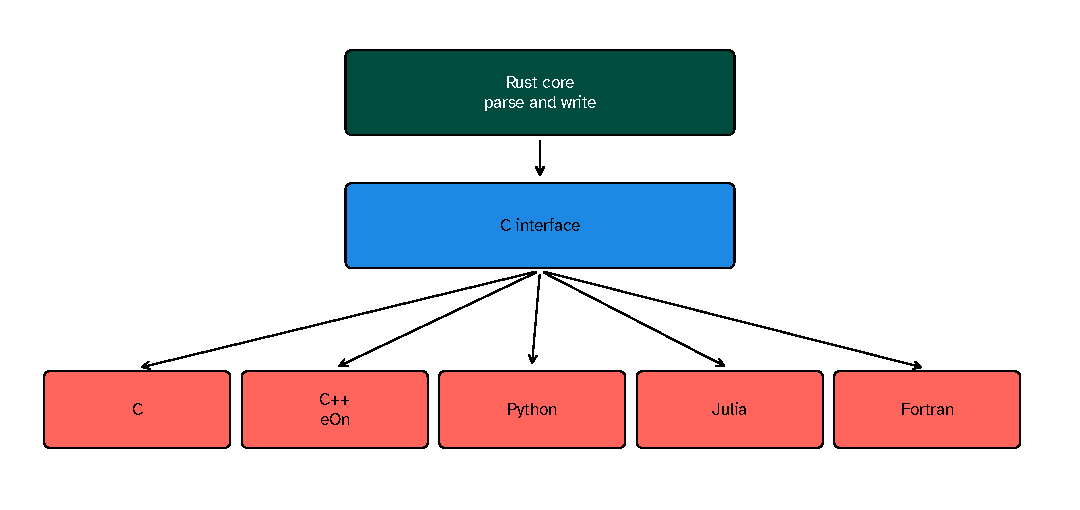
\includegraphics[width=0.92\textwidth]{figures/generated/architecture.pdf}
\caption{The Rust core parses and writes CON.
The C interface is the waist.
eOn 3.6.0 calls the C++ wrapper.}
\label{fig:architecture}
\end{figure}

The caller owns a frame handle and frees it.
Structure-of-arrays accessors return a pointer into that frame.
Absent numeric metadata is a NaN sentinel and is not written back.
The reader records the byte offset of each frame.
The scan that finds those offsets is serial, because each start depends on the counts before it.
Each frame is then parsed on its own, and the frames return in file order.

\begin{lstlisting}[language=Python,caption={A round trip in Python. The default printer preserves binary64. Six decimals are a separate argument.},label={lst:py}]
frames = readcon.read_con("slab.con")
readcon.write_con("rt.con", frames)
\end{lstlisting}

readcon-db is the campaign store for that text \cite{goswamiReadcondbMmapCon2026}.
It writes each CON frame into a memory-mapped store, posts an xxHash3-128 of the text, and keeps secondary indexes on atom count, composition, energy, maximum force and section presence.
A select touches the index and then the frames the index names.
Identical texts share one hash entry, and each frame keeps its own stored text, so the stored blob bytes equal the raw file.
gzip and zstd remain properties of the CON bytes, recognised by content before ingest.
The MPI paths are a single writer, which inserts in global frame order, and a sharded ingest.
Section \ref{sec:perf-mpi} measures both.
The map starts at 2 GiB.
The caller can raise that limit, and a write that fills the map grows it and retries.
Section \ref{sec:performance} names the versions that were clocked.

\section{Case studies}
\label{sec:cases}
Every route below uses one protocol on readcon-core~\readconversion{}.
The build is commit~\readconcommitshort{}.
Table~\ref{tab:params} lists the constants held fixed for every completed route.
An EMT Pt(100) slab, three layers of \(3\times3\), has its bottom layer held on every axis and one adatom held in \(z\).
The adatom hops between neighbouring hollows.
Endpoints were relaxed to \(0.002\,\mathrm{eV/\text{\AA}}\).

\begin{table}[ht]
\centering
\small
\caption{Parameters held fixed for the climbing-image case study and the peer timings.}
\label{tab:params}
\begin{tabular}{llll}
\toprule
Symbol & Meaning & Configuration key & Value \\
\midrule
\(f_{\mathrm{end}}\) & endpoint force tolerance & minimise \texttt{fmax} & \(0.002\,\mathrm{eV/\AA}\) \\
\(f_{\mathrm{band}}\) & band force tolerance & NEB \texttt{fmax} & \(0.01\,\mathrm{eV/\AA}\) \\
\(N_{\mathrm{img}}\) & movable images & NEB images & 5 \\
\(\Delta s\) & steepest-descent step & NEB step size & \(0.1\,\text{\AA}\) \\
\(N_{\mathrm{cap}}\) & iteration cap & NEB max iterations & 4000 \\
\(N_{\mathrm{pair}}\) & peer timing pairs & campaign repeats & 30 \\
\(N_{\mathrm{boot}}\) & BCa resamples & bootstrap draws & 9999 \\
\bottomrule
\end{tabular}
\end{table}
A climbing-image band of five movable images uses the improved tangent \cite{henkelmanClimbingImageNudged2000,henkelmanImprovedTangentEstimate2000} and fixed-step steepest descent on the projected force.
Steepest descent stores no step history, so a difference after the resume comes from the file.
The band is interrupted after 25 steps, written, read back, and resumed to \(0.01\,\mathrm{eV/\text{\AA}}\).
Uninterrupted, it converges in 60 steps with barrier \(0.644561366\,\mathrm{eV}\) and 56 free modes on the middle image.
Table \ref{tab:restartfmt} is every completed route.
Figure \ref{fig:restartfmt} is three of those bands.
Table \ref{tab:restart-pairs} is the 25 writer-reader pairs among Python, C, C++, Fortran and Julia. Each pair reads the restart file written by the other.

% Written by paper/cpc/scripts/gen_cloud_tables.py.
\begin{table}[ht]
\centering
\scriptsize
\caption{Climbing-image band of the EMT Pt(100) hop, stopped after 25 steepest-descent steps, written and read back, then resumed to $0.01\,\mathrm{eV}/\text{\AA}$. File is the largest coordinate change on that round trip. Modes are the free Cartesian degrees of freedom of the middle image (56 when the masks survive). $\Delta E^\ddagger$ and the displacement are against the uninterrupted band, whose barrier is $0.644561366\,\mathrm{eV}$. Force calls are the number of climbing-image ``get\_forces`` evaluations on the timed leg; wall is the median wall-clock seconds of that leg from \texttt{restart\_walls.csv} (\texttt{pixi run cpc-restart-walls}). \textsuperscript{a}Not converged at 4000 steps. The 25 language pairs are Table~\ref{tab:restart-pairs}.}
\label{tab:restartfmt}
\setlength{\tabcolsep}{2.5pt}
\resizebox{\textwidth}{!}{%
\begin{tabular}{@{}lcccccccc@{}}
\toprule
Route & File (\AA) & Modes & Steps & Force calls & Wall (s) & $\Delta E^\ddagger$ (eV) & Max displacement (\AA) \\
\midrule
uninterrupted & -- & 56 & 60 & 61 & 0.575 & $0$ & $0$ \\
CON 3.1, shortest round trip & 0 & 56 & 60 & 36 & 0.603 & $-2.31\times10^{-14}$ & $3.55\times10^{-15}$ \\
CON 3.1, six decimals & $4.90\times10^{-7}$ & 56 & 60 & 36 & 0.602 & $1.19\times10^{-8}$ & $5.69\times10^{-7}$ \\
CON 3.1 read by the ASE eon reader & 0 & 54 & 4000\textsuperscript{a} & 3976 & 32.419 & $-3.52\times10^{-1}$ & $5.43\times10^{0}$ \\
same, periodicity restored by hand & 0 & 54 & 127 & 103 & 1.206 & $-2.93\times10^{-6}$ & $4.21\times10^{-2}$ \\
extended XYZ (ASE) & $5.00\times10^{-9}$ & 56 & 60 & 36 & 0.656 & $1.09\times10^{-9}$ & $4.94\times10^{-9}$ \\
ASE trajectory & 0 & 56 & 60 & 36 & 0.608 & $-2.31\times10^{-14}$ & $3.55\times10^{-15}$ \\
POSCAR (ASE) & $4.90\times10^{-17}$ & 57 & 98 & 74 & 0.903 & $-7.02\times10^{-2}$ & $1.60\times10^{-1}$ \\
legacy CON (ASE eon writer) & \multicolumn{7}{l}{no file: a per-axis constraint is rejected} \\
ASE trajectory, id array & 0 & 56 & 60 & 36 & 0.608 & $-2.31\times10^{-14}$ & $3.55\times10^{-15}$ \\
H5MD MDAnalysis to MDAnalysis & $4.60\times10^{-7}$ & 84 & 97 & 73 & 0.995 & $-7.07\times10^{-2}$ & $1.43\times10^{-1}$ \\
H5MD MDAnalysis to h5py & $4.60\times10^{-7}$ & 56 & 60 & 36 & 0.652 & $-1.98\times10^{-7}$ & $3.67\times10^{-7}$ \\
H5MD h5py to h5py & 0 & 56 & 60 & 36 & 0.630 & $-2.31\times10^{-14}$ & $3.55\times10^{-15}$ \\
H5MD h5py to MDAnalysis & $4.60\times10^{-7}$ & 84 & 97 & 73 & 0.982 & $-7.07\times10^{-2}$ & $1.43\times10^{-1}$ \\
\bottomrule
\end{tabular}}
\end{table}


The shortest CON round trip changes no coordinate.
The barrier moves by \(-2.31\times10^{-14}\,\mathrm{eV}\) and the images by at most \(3.55\times10^{-15}\,\text{\AA}\).
Each of the 25 pairs finishes at that same shift, in 60 steps, with 56 modes.
Six decimals move the file by \(4.90\times10^{-7}\,\text{\AA}\) and the images by \(5.69\times10^{-7}\,\text{\AA}\).
The barrier is \(0.644561378\,\mathrm{eV}\), a shift of \(1.19\times10^{-8}\,\mathrm{eV}\).
The band converges in 60 steps with 56 modes.
Extended XYZ moves the file by \(5.00\times10^{-9}\,\text{\AA}\) and the barrier by \(+1.09\times10^{-9}\,\mathrm{eV}\), with the same step count and the same mode count.
The ASE trajectory matches the language-pair floor.
An extra identifier array on that trajectory does not survive the round trip, and the mode count stays 56 because the mask does.

POSCAR moves the file by \(4.90\times10^{-17}\,\text{\AA}\) and drops the height constraint, so the middle image has 57 free modes.
The band converges in 98 steps, \(0.160\,\text{\AA}\) away, with a barrier \(7.02\times10^{-2}\,\mathrm{eV}\) lower.
That is the \(70.2\,\mathrm{meV}\) in the abstract.
The ASE eon writer produces no file, because a per-axis constraint is not a constraint that writer emits.
The ASE eon reader keeps 54 modes, runs to the 4000-step cap without converging, and finishes \(0.352\,\mathrm{eV}\) and \(5.43\,\text{\AA}\) away.
Restoring periodicity by hand leaves the mask collapse in place: 54 modes, 127 steps, a barrier shift of \(-2.93\times10^{-6}\,\mathrm{eV}\), and a displacement of \(4.21\times10^{-2}\,\text{\AA}\).

The H5MD block in the table is a second measurement, distinct from the survey row.
The writer attaches a Boolean \(N\times3\) mask array, an identifier array, the velocity unit \(\text{\AA}\,\mathrm{ps}^{-1}\), and the boundary periodic, periodic, none.
MDAnalysis reading that file, whether it wrote the file or h5py did, returns 84 free modes and a barrier \(7.07\times10^{-2}\,\mathrm{eV}\) lower, with a file shift of \(4.60\times10^{-7}\,\text{\AA}\).
The mode count is the loss of the mask and the identifier.
h5py reading the MDAnalysis file keeps 56 modes, finishes in 60 steps, and moves the barrier by \(-1.98\times10^{-7}\,\mathrm{eV}\).
h5py reading its own file is bit-exact and lands on the language-pair floor.
The coordinate gap between the two files is the single-precision write.

\begin{figure}[ht]
\centering
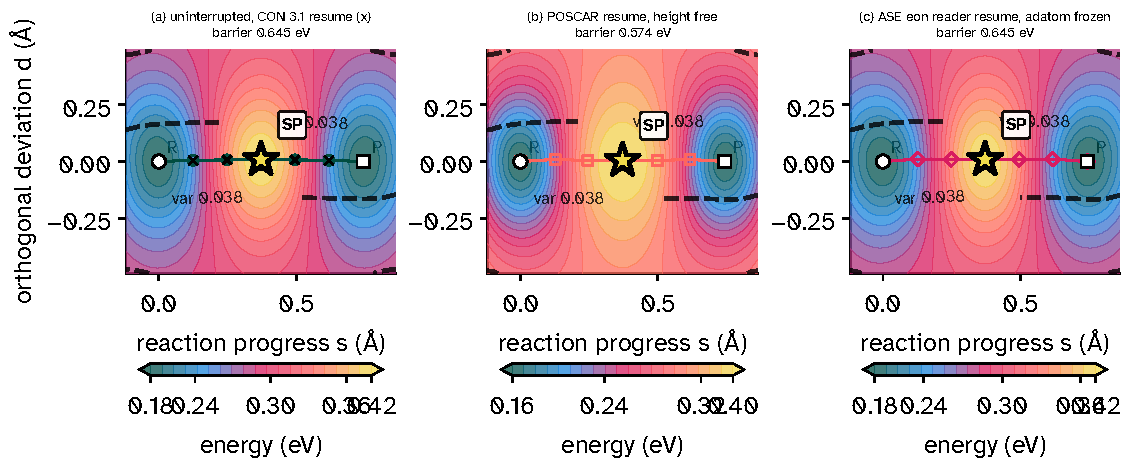
\includegraphics[width=\textwidth]{figures/generated/restart_formats.pdf}
\caption{Resumed climbing-image bands of the EMT Pt(100) hop on the \((s, d)\) plane \cite{goswamiTwodimensionalRmsdProjections2026}.
Each panel is the energy surface of its own band.
(a) Uninterrupted, with the CON 3.1 resume as crosses.
(b) POSCAR, height constraint dropped.
(c) ASE eon reader with periodicity restored by hand.
The routes differ in barrier and in free modes, as Table \ref{tab:restartfmt} records.}
\label{fig:restartfmt}
\end{figure}

\subsection{The mask and the prefactor}
The symmetric hop can sit on the straight line, so a lost lateral constraint need not move the barrier by much.
The same 28-atom Pt(100) \(3\times3\times3\) slab, seven images in all, was then converged with FIRE to \(0.01\,\mathrm{eV/\text{\AA}}\) instead of steepest descent \cite{bitzekStructuralRelaxationMade2006}.
ASE 3.29.0 has no eOn Morse calculator in this run, so the relaxation, the band and the Hessian use EMT.
With the height held, the barrier is \(0.36659812266626624\,\mathrm{eV}\) on a path of \(2.9004016648060382\,\text{\AA}\).
The middle image has 56 free modes and one imaginary mode, \(-4.076276454192005\,\mathrm{meV}\), with \(0.9872893953755115\) of its weight on the adatom's lateral motion.
The Vineyard prefactor of that Hessian is \(3.2438730218892426\times10^{10}\,\mathrm{Hz}\) \cite{vineyardFrequencyFactorsIsotope1957}.
FIRE took 26 steps and then 16 climbing steps.

The ASE eon reader turns the height-held column into a full freeze, so the adatom is fixed on every axis.
The default interpolation then stops because the constraints change the path, and the band was built with the constraints ignored during interpolation.
FIRE took 26 steps and then 14 climbing steps, reached \(0.007095\,\mathrm{eV/\text{\AA}}\), and left the adatom on the straight interpolation.
The relative peak is \(0.3665836803750313\,\mathrm{eV}\) on a path of \(2.9595547559012947\,\text{\AA}\).
The middle image has 54 free modes and no imaginary mode, so the Vineyard ratio is undefined.
Figure \ref{fig:asemask} is the two bands.
The barriers differ in the fifth digit.
The prefactor exists for one reading and does not exist for the other.

\begin{figure}[ht]
\centering
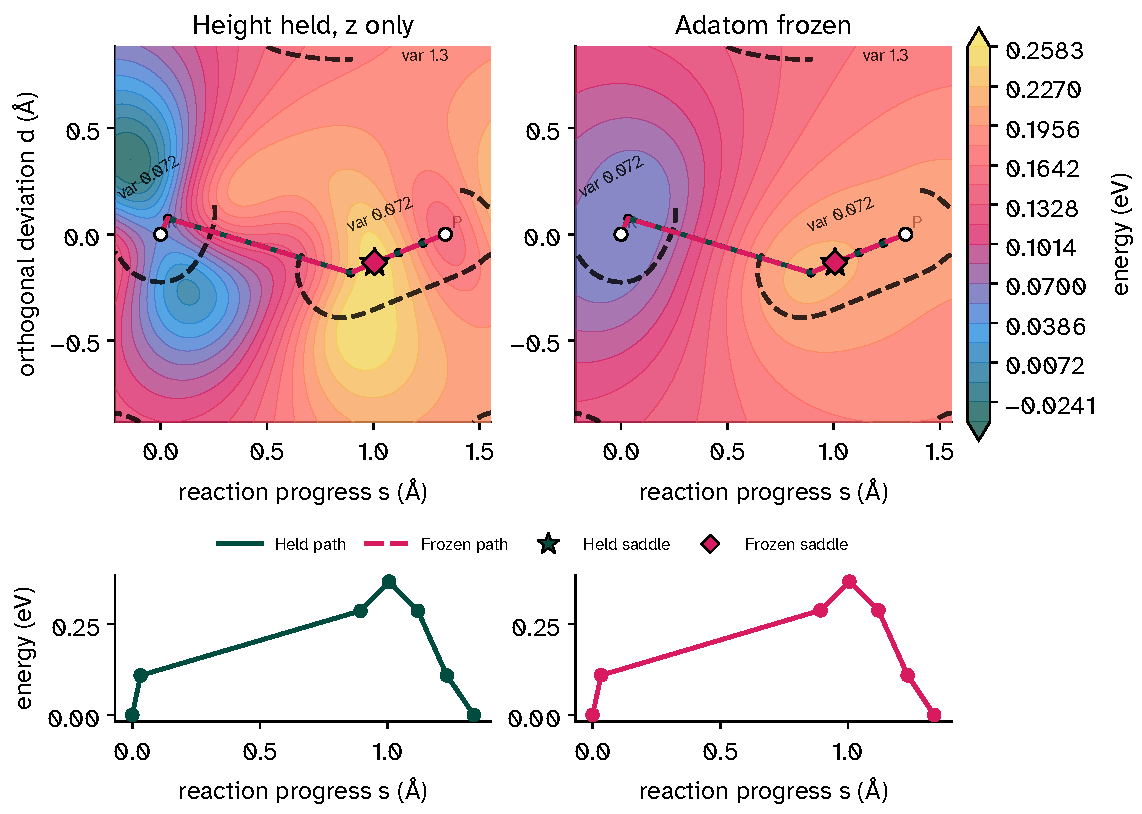
\includegraphics[width=\textwidth]{figures/generated/ase_mask.pdf}
\caption{EMT climbing-image bands for a Pt adatom hop on Pt(100), each mask on its own \((s, d)\) map \cite{goswamiTwodimensionalRmsdProjections2026}.
Height held: \(0.366598\,\mathrm{eV}\), 56 free modes, one imaginary mode.
ASE eon reading: \(0.366584\,\mathrm{eV}\), 54 free modes, no imaginary mode.}
\label{fig:asemask}
\end{figure}

\subsection{eOn resuming a Morse band}
An eOn 3.6.0 client ran a Morse Pt potential on a 28-atom slab, bottom atoms at mask 7, five movable images, steepest descent \cite{rohitgoswamiTheochemuieonV3602026}.
The band section selects the optimiser.
This run sets steepest descent there.
When the total number of optimiser steps matches, the shortest round trip reproduces the uninterrupted barrier, \(0.63493\,\mathrm{eV}\), with barrier difference 0 and a largest minimum-image displacement of \(8.881784197001252\times10^{-15}\,\text{\AA}\).
Six decimals give barrier \(0.634931\,\mathrm{eV}\) and a largest minimum-image displacement of \(4.918050526825368\times10^{-7}\,\text{\AA}\).
Figure \ref{fig:restart} is that comparison.
Section \ref{sec:supp-restart} gives the per-image displacement.

A control file left the default band optimiser in place.
Both printers of that control finish at \(0.670723\,\mathrm{eV}\).
The uninterrupted barrier in the same file is \(0.63361\,\mathrm{eV}\), so the difference is \(0.037113\,\mathrm{eV}\).
The two printers agree with each other.
They do not agree with the uninterrupted barrier, because the checkpoint does not carry the optimiser history.

A dimer started from the round-trip geometry stops for the same reason as the uninterrupted dimer, too many iterations.
Both report saddle energy \(-112.618941\,\mathrm{eV}\) and curvature \(-10.613681\).
Six decimals give \(-112.618944\,\mathrm{eV}\) and \(-10.613677\), an energy shift of \(-3\times10^{-6}\,\mathrm{eV}\).
The comparison is of the stopped search.

\begin{figure}[ht]
\centering
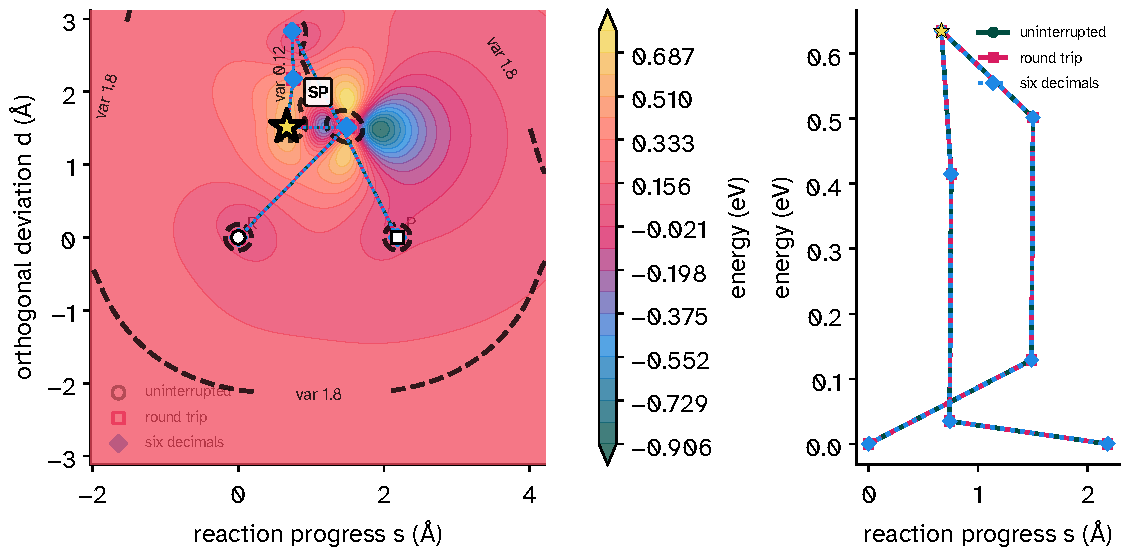
\includegraphics[width=\textwidth]{figures/generated/restart.pdf}
\caption{Final images of the Morse band on the \((s, d)\) plane \cite{goswamiTwodimensionalRmsdProjections2026}.
With the step count matched, the shortest round trip returns the uninterrupted barrier, \(0.63493\,\mathrm{eV}\).
The colour bar is the fitted surface.
The image energies are the energy column of the uninterrupted band, and the highest image is \(0.634930\,\mathrm{eV}\).}
\label{fig:restart}
\end{figure}

\subsection{The velocity unit and identity}
On the 28-atom slab the kinetic energy is \(0.8878595057627452\,\mathrm{eV}\) in the natural unit and \(92.0201533142073\,\mathrm{eV}\) when those numbers are read as \(\text{\AA}/\mathrm{fs}\).
The ratio is \(103.64269652680504\), the square of \(10.180505710759414\,\mathrm{fs}\).
One velocity Verlet step of \(1\,\mathrm{fs}\) then moves the atoms by an RMSD of \(0.09556596694568728\,\text{\AA}\), maximum \(0.31544697368347396\,\text{\AA}\) \cite{swopeComputerSimulationMethod1982}.
On a separate \(10{,}001\)-atom slab at \(300\,\mathrm{K}\) the logged kinetic energy is \(390.085819\,\mathrm{eV}\) and the value obtained by reading those numbers as \(\text{\AA}/\mathrm{fs}\) is \(40429.545793\,\mathrm{eV}\).
Section \ref{sec:supp-velocity} plots the step.

The public HCN and HNC endpoints are frames 0 and 1 of one file \cite{vanmourikAbInitioGlobal2001,goswamiReproducibleOrchestrationBest2026}.
On both, readcon-core returns masks \texttt{000 000 000}, identifiers \texttt{0 1 2}, and the declared natural unit.
Frame 2 is a constructed probe, not a public endpoint: masks \texttt{000 000 100} and identifiers \texttt{2 0 1}, with hydrogen fixed on \(x\) only.
The ASE eon reader stops on the velocity block of that file.
Given the probe coordinates alone, it returns the three atoms as free, free, and fixed on every axis, and it returns no identifiers.
Table \ref{tab:hcn} is that split.

\input{figures/generated/hcn_table}

\section{Performance}
\label{sec:performance}
Timings below are medians.
Where an interval is reported, it is a bias-corrected and accelerated 95 percent interval of the median from 9999 resamples \cite{efronBetterBootstrapConfidence1987}.
The host, the compiler and the thread pin are part of the result \cite{kaliberaRigorousBenchmarkingReasonable2013,hoeflerScientificBenchmarkingParallel2015}.
Parallel runs are compared at fixed work or fixed work per rank.
This section names the build that was clocked.

Thread timings and peer campaigns used an Intel(R) Xeon(R) Processor, family 6, model 173, 8 hardware threads at \(2700\,\mathrm{MHz}\), \(49{,}342{,}768\,\mathrm{kB}\) of memory, Ubuntu 24.04, Linux 6.12.94+, rustc 1.88.0, g++ 13.3.0 (Ubuntu 13.3.0-6ubuntu2~24.04.1) and Python 3.12.3.
The MPI campaign used an Intel(R) Xeon(R) Processor, family 6, model 207, stepping 2, 8 cores, 1 thread per core, 1 socket, \(49{,}342{,}904\,\mathrm{kB}\) of memory, Linux 6.12.94+, rustc 1.99.0, GCC 13.3.0 (Ubuntu 13.3.0-6ubuntu2~24.04.1) and MPICH 4.2.3; the campaign log records BogoMIPS \(4800.00\) and no CPU MHz, so no clock frequency is printed for that host.
The store campaign used an Intel(R) Xeon(R) Processor, 8 CPUs, \(47.07\,\mathrm{GiB}\), Python 3.12.3 and rustc 1.88.0; that log records neither CPU family, model id, nor MHz.

\subsection{Threads}
\label{sec:perf-read}
The file holds \(10{,}000\) copies of one 218-atom frame, \(167{,}710{,}000\) bytes.
readcon-core 0.17.2, built with rustc 1.88.0, reads it.
OpenMP and BLAS are pinned to one thread outside the pool under test.
Table \ref{tab:perf} is the warm-cache read.
The native Rust pool finishes in \(0.096961\,\mathrm{s}\), \(1730\,\mathrm{MB/s}\), \(103134\) frames/s, which is \(9.70\,\mu\mathrm{s}\) per frame.
The C++ wrapper eOn calls finishes in \(0.102333\,\mathrm{s}\).
The median of the paired Rust-to-C++ ratios is \(0.942\), with interval \([0.933, 0.992]\).
That interval belongs to the paired ratios, not to the quotient of the two medians just given.
At one thread the medians are \(0.249621\,\mathrm{s}\) and \(0.260032\,\mathrm{s}\), and the median of the paired ratios is \(0.963\).
Building a Python object per frame takes \(0.879852\,\mathrm{s}\).
One EMT force call on this host has median \(5.200\times10^{-5}\,\mathrm{s}\), so the native read of the whole file is \(1864.6\) such calls.
The in-process Morse timing from the band study is \(3.036\times10^{-4}\,\mathrm{s}\) per call, and the same file is \(319.4\) of those calls.

\begin{table}[ht]
\centering
\small
\caption{Warm read of \(10{,}000\) frames, \(167{,}710{,}000\) bytes, readcon-core 0.17.2.
Native rows are 15 repeats.
The Python row is 9 repeats.
The interval is a bias-corrected and accelerated 95 percent interval of the median.}
\label{tab:perf}
\begin{tabular}{lrrl}
\toprule
Reader & Median (s) & MB/s & Interval (s) \\
\midrule
Rust, automatic pool & 0.096961 & 1730 & [0.095046, 0.099329] \\
C++ wrapper, automatic pool & 0.102333 & 1639 & [0.095919, 0.106351] \\
Rust, 1 thread & 0.249621 & 671.9 & [0.238949, 0.253467] \\
C++ wrapper, 1 thread & 0.260032 & 645.0 & [0.245996, 0.269355] \\
Python, full objects & 0.879852 & 190.6 & [0.857167, 1.393448] \\
\bottomrule
\end{tabular}
\end{table}

A separate five-repeat sweep on the same file sets the pool size.
The printed speedups are medians of the paired one-thread/eight-thread ratios, each with its bias-corrected and accelerated 95 percent BCa interval from \texttt{e2\_speedup\_bca.json} (\texttt{pixi run cpc-e2-speedup-bca}); they are not the quotients of the two endpoint medians.
Rust goes from \(0.24435\,\mathrm{s}\) at one thread to \(0.08695\,\mathrm{s}\) at eight; the paired-ratio median is \(2.84\) with BCa interval \([2.67, 3.08]\).
C++ goes from \(0.24929\,\mathrm{s}\) to \(0.09113\,\mathrm{s}\); the paired-ratio median is \(2.66\) with BCa interval \([2.63, 2.76]\).
Python full objects go from \(0.9033\,\mathrm{s}\) to \(0.8209\,\mathrm{s}\); the paired-ratio median is \(1.14\) with BCa interval \([0.84, 1.18]\).
Section \ref{sec:supp-threads} records the thirty-pair Python sweep from the earlier campaign.
Hashes of the returned fields at 1, 2, 3, 4 and 8 threads are identical.
Figure \ref{fig:layers} is the automatic-pool rates.
Figure \ref{fig:roofline} places the five-repeat scaling rates under the memory-copy rate.
No Amdahl curve is drawn.
The in-process file read is \(0.090867964\,\mathrm{s}\) and the boundary scan is \(0.034595311\,\mathrm{s}\).
Their sum, \(0.125463275\,\mathrm{s}\), is \(0.502615\) of the 15-repeat one-thread median \(0.249621235\,\mathrm{s}\).
That quotient is not a serial fraction of the five-repeat sweep.

\begin{figure}[ht]
\centering
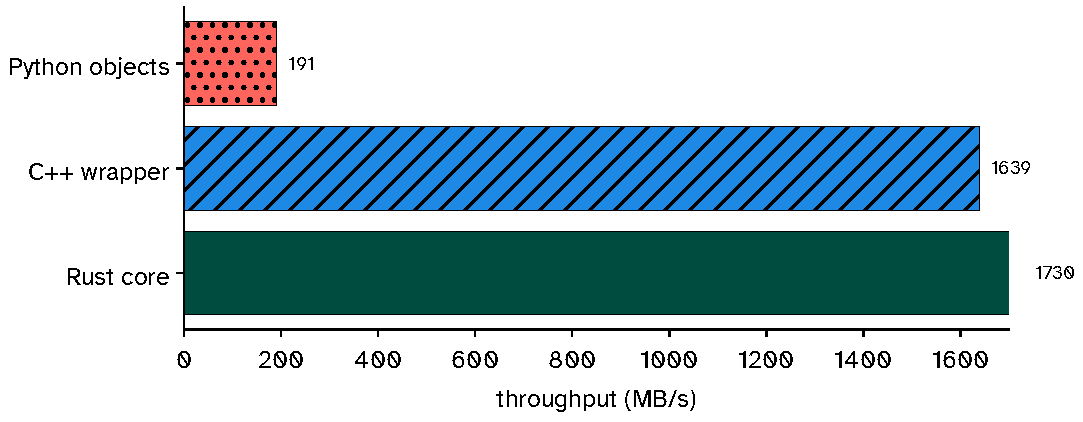
\includegraphics[width=0.72\textwidth]{figures/generated/layers.pdf}
\caption{Warm-cache rate for the automatic Rust pool, the C++ wrapper and the Python full-object read, from the medians in Table \ref{tab:perf}.}
\label{fig:layers}
\end{figure}

\begin{figure}[ht]
\centering
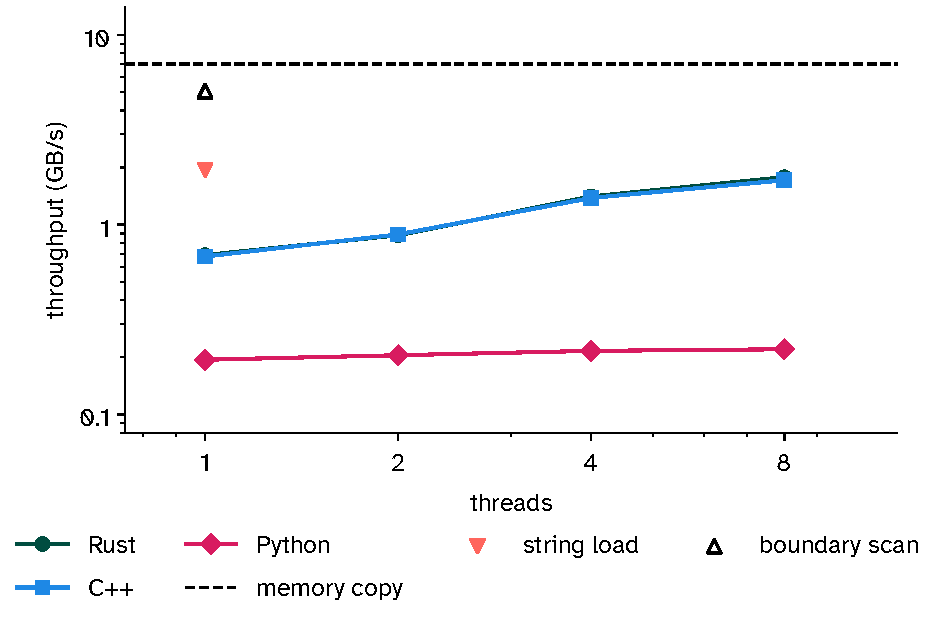
\includegraphics[width=0.85\textwidth]{figures/generated/roofline.pdf}
\caption{Five-repeat scaling rates for Rust, C++ and Python on readcon-core 0.17.2.
The dashed line is the hot-cache copy, \(5.78\,\mathrm{GB/s}\).
The triangles are the 15-repeat file-read and boundary-scan rates.
They are not an Amdahl curve for the scaling points.}
\label{fig:roofline}
\end{figure}

\subsection{Peers}
\label{sec:perf-peers}
Table \ref{tab:peers} is the fairness campaign on readcon-core~\readconversion{} (commit~\readconcommitshort{}) and rustc 1.88.0 on the family-6 model-173 host named above.
Thirty interleaved pairs compare a full-field Python read and a coordinates-only accumulation against chemfiles XYZ, h5py and MDAnalysis H5MD.
On \(10{,}000\) frames the full-field ratios are \(1.73\) against chemfiles, \(51.9\) against h5py and \(0.154\) against MDAnalysis H5MD; the coordinates-only accumulation changes those ratios to \(1.63\), \(36.4\) and \(0.160\).
Those six numbers are Table~\ref{tab:peers} and the abstract; the driver is \texttt{pixi run cpc-fairness}.
Table \ref{tab:peers-ab} is the separate campaign-A and campaign-B survey against ASE eon, chemfiles, h5py, MDAnalysis, ASE extended XYZ and the ASE trajectory on the same host.
Campaign A reports \(0.253\) against ASE eon, \(1.58\) against chemfiles, \(47.6\) against h5py and \(0.160\) against MDAnalysis H5MD on the long file.
Campaign B reproduces the ASE eon ratio at \(0.257\) and adds ASE extended XYZ (\(0.251\)) and the ASE trajectory (\(0.774\) on the long file, \(2.95\) on one slab).
Absolute readcon-core medians are \(0.935\,\mathrm{s}\) in B and \(0.914\,\mathrm{s}\) in A.
Section \ref{sec:appendix-peers} extends campaign A to the 1-frame and 100-frame files.
On one frame the open dominates, and h5py and chemfiles lose the lead they have on the long file.

% Fairness campaign: full_fields vs coords_accum. Generated for v7.7 from ratios_v76_fairness.csv.
\begin{table}[ht]
\centering
\small
\caption{Paired ratios of the one-worker Python readcon-core time to each peer on \(10{,}000\) frames, so a value below 1 means readcon-core finished sooner.
Each cell is 30 interleaved pairs; the interval is the median of those paired ratios with its bias-corrected and accelerated 95 percent BCa interval.
Mode \texttt{full\_fields} keeps the parsed frames (mask, identifier, cell and periodic flags available).
Mode \texttt{coords\_accum} runs the same parse and then accumulates only the first atom's \(x+y+z\).
Peers return chemfiles XYZ coordinates, one h5py numeric array, or MDAnalysis H5MD coordinates.
The driver is \texttt{paper/cpc/bench/run\_fairness.py} (\texttt{pixi run cpc-fairness}).}
\label{tab:peers}
\footnotesize
\setlength{\tabcolsep}{4pt}
\begin{tabular}{lllrl}
\toprule
Mode & Peer & Fields & Ratio & Interval \\
\midrule
full\_fields & chemfiles XYZ & coordinates & 1.73 & [1.72, 1.77] \\
full\_fields & h5py & one binary array & 51.9 & [51.0, 53.9] \\
full\_fields & MDAnalysis H5MD & coordinates & 0.154 & [0.151, 0.164] \\
coords\_accum & chemfiles XYZ & coordinates & 1.63 & [1.61, 1.65] \\
coords\_accum & h5py & one binary array & 36.4 & [32.8, 37.2] \\
coords\_accum & MDAnalysis H5MD & coordinates & 0.160 & [0.157, 0.164] \\
\bottomrule
\end{tabular}
\end{table}


\begin{figure}[ht]
\centering
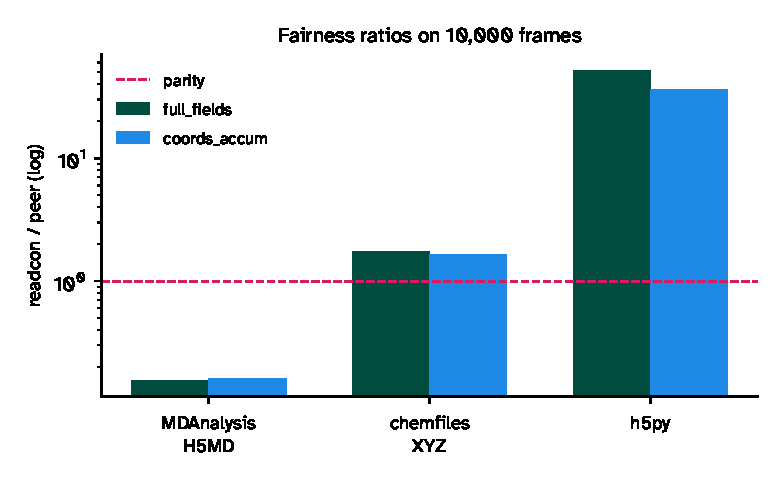
\includegraphics[width=0.72\textwidth]{figures/generated/fairness_ratios.pdf}
\caption{Fairness ratios from Table~\ref{tab:peers}: readcon-core time over peer time on \(10{,}000\) frames for \texttt{full\_fields} and \texttt{coords\_accum}.
Values below the dashed line are wins for readcon-core.}
\label{fig:fairness}
\end{figure}

% Campaign A / B peer survey. Wall times are medians from ratios.csv and repeats_v76_b.csv.
\begin{table}[ht]
\centering
\small
\caption{Campaign A and B peer ratios on the same host (family 6, model 173, \(2700\,\mathrm{MHz}\)), thirty interleaved pairs each.
Wall columns are median wall-clock seconds from the committed repeat CSVs (\texttt{ratios.csv}, \texttt{repeats\_v76\_b.csv}).
The evaluation count on the long file is \(10{,}000\) frames; the slab rows are one frame.
Campaign B adds ASE extended XYZ and the ASE trajectory; its ASE eon ratio on the \(10{,}000\)-frame file is \(0.257\) against \(0.253\) in A.
These rows are not the fairness modes of Table~\ref{tab:peers}.}
\label{tab:peers-ab}
\scriptsize
\setlength{\tabcolsep}{2pt}
\resizebox{\textwidth}{!}{%
\begin{tabular}{lllrrrl}
\toprule
Payload & Peer & Fields & readcon (s) & peer (s) & Ratio & Interval \\
\midrule
10000 frames & ASE eon & same CON text & 0.914 & 3.614 & 0.253 & [0.251, 0.256] \\
10000 frames & chemfiles XYZ & coordinates & 0.886 & 0.563 & 1.58 & [1.57, 1.6] \\
10000 frames & h5py & one binary array & 0.993 & 0.0208 & 47.6 & [46.7, 48.5] \\
10000 frames & MDAnalysis H5MD & coordinates & 0.930 & 5.844 & 0.160 & [0.157, 0.162] \\
Pt slab & ASE eon & same CON text & 0.00215 & 0.00993 & 0.215 & [0.211, 0.218] \\
Pt slab & chemfiles XYZ & coordinates & 0.00212 & 0.00204 & 1.04 & [1.03, 1.04] \\
Pt slab & h5py & one binary array & 0.00213 & 0.000521 & 4.1 & [4.06, 4.13] \\
Pt slab & MDAnalysis H5MD & coordinates & 0.00216 & 0.00592 & 0.365 & [0.359, 0.368] \\
10000 frames & ASE extended XYZ & ASE atoms & 0.975 & 3.858 & 0.251 & [0.243, 0.254] \\
10000 frames & ASE trajectory & ASE atoms & 0.956 & 1.233 & 0.774 & [0.761, 0.787] \\
Pt slab & ASE extended XYZ & ASE atoms & 0.00222 & 0.0143 & 0.154 & [0.154, 0.155] \\
Pt slab & ASE trajectory & ASE atoms & 0.00221 & 0.000751 & 2.95 & [2.92, 3.05] \\
\bottomrule
\end{tabular}}
\end{table}


\subsection{MPI}
\label{sec:perf-mpi}
The MPI run used readcon-core 0.17.0 and readcon-db 0.1.8 on the eight-core host named above.
Ranks 16 and 32 were not run.
MPICH 4.2.3 used the ch4:ofi device, bound to cores, with UCX and libfabric on TCP.
Each rank is one thread.
Each cell is five repeats.
Cold repeats drop the page cache.
Warm repeats follow an untimed warmup.
The median is the third of the five sorted times.
Every one of the 480 repeats matched the serial bytes.

Strong scaling holds the file fixed.
The CON file is \(1{,}583{,}691\) copies of a small frame, \(3{,}167{,}382\) frames, \(1{,}073{,}742{,}498\) bytes.
The database file is \(30{,}965\) frames of \(1{,}000\) atoms, ingested four times, with four shards on the sharded path.
Table \ref{tab:mpi-strong} is the warm medians.
Shared read goes from \(9.088\,\mathrm{s}\) to \(1.504\,\mathrm{s}\), a ratio \(6.04\).
Scatter goes from \(9.223\,\mathrm{s}\) to \(1.836\,\mathrm{s}\), ratio \(5.02\).
MPI-IO write goes from \(8.369\,\mathrm{s}\) to \(1.416\,\mathrm{s}\), ratio \(5.91\).
Gather write goes from \(9.490\,\mathrm{s}\) to \(2.152\,\mathrm{s}\), ratio \(4.41\).
One-writer ingest goes from \(31.699\,\mathrm{s}\) to \(16.810\,\mathrm{s}\), ratio \(1.89\).
Four-shard ingest goes from \(32.549\,\mathrm{s}\) to \(18.805\,\mathrm{s}\), ratio \(1.73\).
Cold shared read goes from \(9.904\,\mathrm{s}\) to \(2.113\,\mathrm{s}\).
Figure \ref{fig:mpi-strong} is the warm speedup.
The full rank list, cold and warm, is in Section \ref{sec:supp-mpi}.

\input{figures/generated/mpi_strong_warm}

\begin{figure}[ht]
\centering
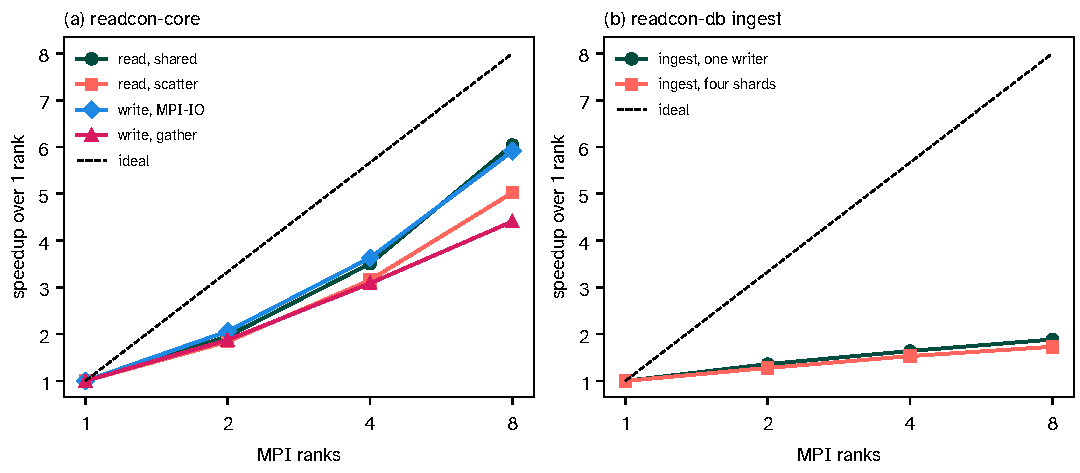
\includegraphics[width=\textwidth]{figures/generated/mpi_strong.pdf}
\caption{Strong-scaling speedup from the warm medians in Table \ref{tab:mpi-strong}.
The dashed line is ideal speedup.
Ranks 1, 2, 4 and 8 on the 8-core host.
Every output matched the serial bytes.}
\label{fig:mpi-strong}
\end{figure}

Weak scaling gives every rank the same frame count as the one-rank run.
readcon-core holds \(400{,}000\) frames per rank.
readcon-db ingests \(7{,}700\) frames of \(1{,}000\) atoms per rank, four copies.
Table \ref{tab:mpi-weak} is the warm medians, and the ratio is the eight-rank time over the one-rank time.
Shared read grows by \(1.36\), scatter by \(1.61\), MPI-IO write by \(1.33\), and gather write by \(1.78\).
One-writer ingest grows by \(3.77\), from \(7.841\,\mathrm{s}\) to \(29.594\,\mathrm{s}\).
Four-shard ingest grows by \(4.68\), from \(7.465\,\mathrm{s}\) to \(34.899\,\mathrm{s}\).
Every rank writes one virtio ext4 device, and the byte count grows with the rank count.
Table \ref{tab:weak-io} is the aggregate rate on that device.
Shared read and MPI-IO write still gain rate from one rank to eight.
Both ingest paths level off, and at eight ranks the sharded path is the slower of the two on the same bytes.
Figure \ref{fig:mpi-weak} is that growth.

\input{figures/generated/weak_io}

\input{figures/generated/mpi_weak_warm}

\begin{figure}[ht]
\centering
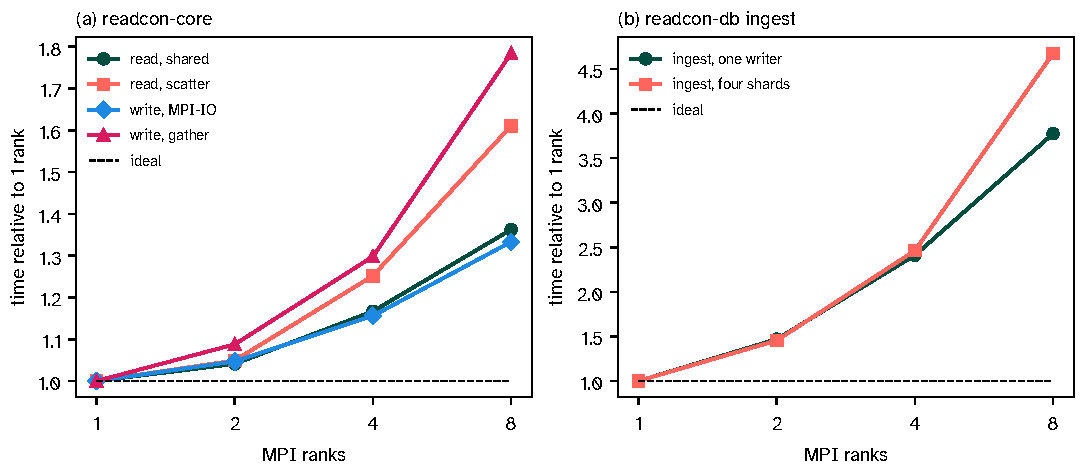
\includegraphics[width=\textwidth]{figures/generated/mpi_weak.pdf}
\caption{Weak scaling from the warm medians in Table \ref{tab:mpi-weak}.
The dashed line is a ratio of 1, the same time as one rank.
The ingest ratios lie above that line.}
\label{fig:mpi-weak}
\end{figure}

\subsection{The store}
\label{sec:perf-db}
The store measurements used readcon-db 0.1.8 and readcon-core 0.16.2 \cite{goswamiReadconcoreV0162Conconvel2026} on the store host named above.
The archived store release is 0.2.0 \cite{goswamiReadcondbMmapCon2026}.
Threads are pinned to 1.
Five repeats are interleaved.
The page cache was not dropped.
A fresh-process query starts a new process with the cache left in place.
A warm query is the next query in that process.
The timed corpora have \(1{,}000\) and \(10{,}000\) frames, and every frame has its own xxHash3-128.
The frames are ASE effective-medium geometries stored as CON text.
Section \ref{sec:appendix-db} records the repeats and the figures.

At \(10{,}000\) frames the ingest medians are \(0.311306\,\mathrm{s}\) for readcon-db (\(32{,}123\) frames/s, \(35.09\,\mathrm{MB/s}\)), \(48.411\,\mathrm{s}\) for ASE's database committing every write (\(206.6\) frames/s), and \(5.985\,\mathrm{s}\) for one ASE connection that still commits every \(5{,}000\) rows (\(1{,}671\) frames/s).
The paired ratios are \(0.006800\) against the per-write commits and \(0.05283\) against the single connection.
At \(10{,}000\) frames the readcon-db fresh-process medians are \(8.14\,\mathrm{ms}\), \(10.1\,\mathrm{ms}\) and \(9.57\,\mathrm{ms}\) for composition, energy and maximum force, and the warm medians are \(0.176\,\mathrm{ms}\), \(0.211\,\mathrm{ms}\) and \(0.208\,\mathrm{ms}\).
ASE's database, on the same three queries, takes \(0.286\,\mathrm{s}\), \(0.223\,\mathrm{s}\) and \(0.225\,\mathrm{s}\) in a fresh process and \(0.258\,\mathrm{s}\), \(0.203\,\mathrm{s}\) and \(0.206\,\mathrm{s}\) warm.
A directory of the same text takes \(0.140\,\mathrm{s}\), \(0.138\,\mathrm{s}\) and \(0.138\,\mathrm{s}\) warm.
readcon-db occupies \(2.503\) times the raw CON text: the text plus the indexes.
The map used for these tables starts at \(2\,\mathrm{GiB}\), so a one-million-frame open exceeds it and stays outside the tables.

\section{Conclusions}
\label{sec:conclusions}
The geometry file in a rare-event campaign is the restart state of the search.
The resume reads a per-axis mask, a persistent identifier, a declared time unit, binary64 coordinates with their periodic flags, and a version two readers agree on.
On one masked slab, every common format tested here drops at least one of those fields.
The ASE POSCAR resume drops the height constraint and finishes \(70.2\,\mathrm{meV}\) lower.
Five extended XYZ readers return four answers for one file.
CON 3.1 states the grammar and the corpus decides the listed files.
The conformance goldens are Python, C, Fortran and Julia.
Twenty-five writer-reader pairs run one parser from Python, C, C++, Fortran and Julia.
They finish at the same barrier, \(0.644561366\,\mathrm{eV}\).
With the height held, the Vineyard prefactor of the EMT hop is \(3.2438730218892426\times10^{10}\,\mathrm{Hz}\).
The ASE eon reading of the same band has no imaginary mode, so that ratio is undefined.
A warm read of \(10{,}000\) frames of 218 atoms takes \(9.70\,\mu\mathrm{s}\) per frame on the 0.17.2 build named in Section \ref{sec:performance}.
On that file a full-field Python read finishes at \(0.154\) times MDAnalysis H5MD, \(1.73\) times chemfiles XYZ and \(51.9\) times h5py; coordinate accumulation alone changes those ratios to \(0.160\), \(1.63\) and \(36.4\).
Shared MPI reads speed up by \(6.04\) from one rank to eight on this host.
Under weak scaling the four-shard ingest grows by \(4.68\) because every rank writes the same device.

\section*{Data availability}
\label{sec:data}
\setlength{\emergencystretch}{2em}
The release measured here is readcon-core~\readconversion{} at commit
\begin{center}
\url{\readconcommit}.
\end{center}
The version DOI waits on the 0.17.2 deposit; the source placeholder is \texttt{\readcondoi}.
The concept record is
\url{https://doi.org/10.5281/zenodo.18753567}
\cite{goswamiReadconcoreConConvel2026}.
readcon-core 0.16.2, used for the store timings, is
\url{https://doi.org/10.5281/zenodo.23264985}
\cite{goswamiReadconcoreV0162Conconvel2026}.
The companion store is archived at
\url{https://doi.org/10.5281/zenodo.23652386}
\cite{goswamiReadcondbMmapCon2026}.
The archived tree at that commit regenerates every number in this paper.
The ten-thousand-frame timing file is rebuilt by repeating
\path{resources/test/cuh2.con} into
\path{paper/cpc/bench/work/frames-10000.con}.
Section~6 is rebuilt by \texttt{python}
\path{paper/cpc/data/cloud-runs-2/cloud-run/run_05.py}
with \texttt{READCON\_CORE\_ROOT} at that commit.
Table~\ref{tab:peers} is rebuilt by \texttt{pixi run cpc-fairness}.
The thread speedup BCa intervals are rebuilt by \texttt{pixi run cpc-e2-speedup-bca}.
The specification, the grammar, the corpus and the campaign results are the supplementary material.

\section*{CRediT authorship contribution statement}
\label{sec:credit}
Rohit Goswami: Conceptualization, Methodology, Software, Visualization, Writing -- original draft, Writing -- review and editing.

\section*{Declaration of competing interest}
\label{sec:competing}
The authors declare that they have no known competing financial interests or personal relationships that could have appeared to influence the work reported in this paper.

\section*{Acknowledgements}
\label{sec:acknowledgements}
The author's family, and the pets who share the house, carried the ordinary days while this was written.
Ruhila Goswami designed the colour palette used for every figure.

\bibliographystyle{elsarticle-num}
\bibliography{rg_main}
\end{document}
